\subsection*{SAR: MFP and \% Inhibition HCT-116}
\begin{figure}[htbp!] % 'h' places the figure approximately here
	\centering
	\hspace{-1cm}
	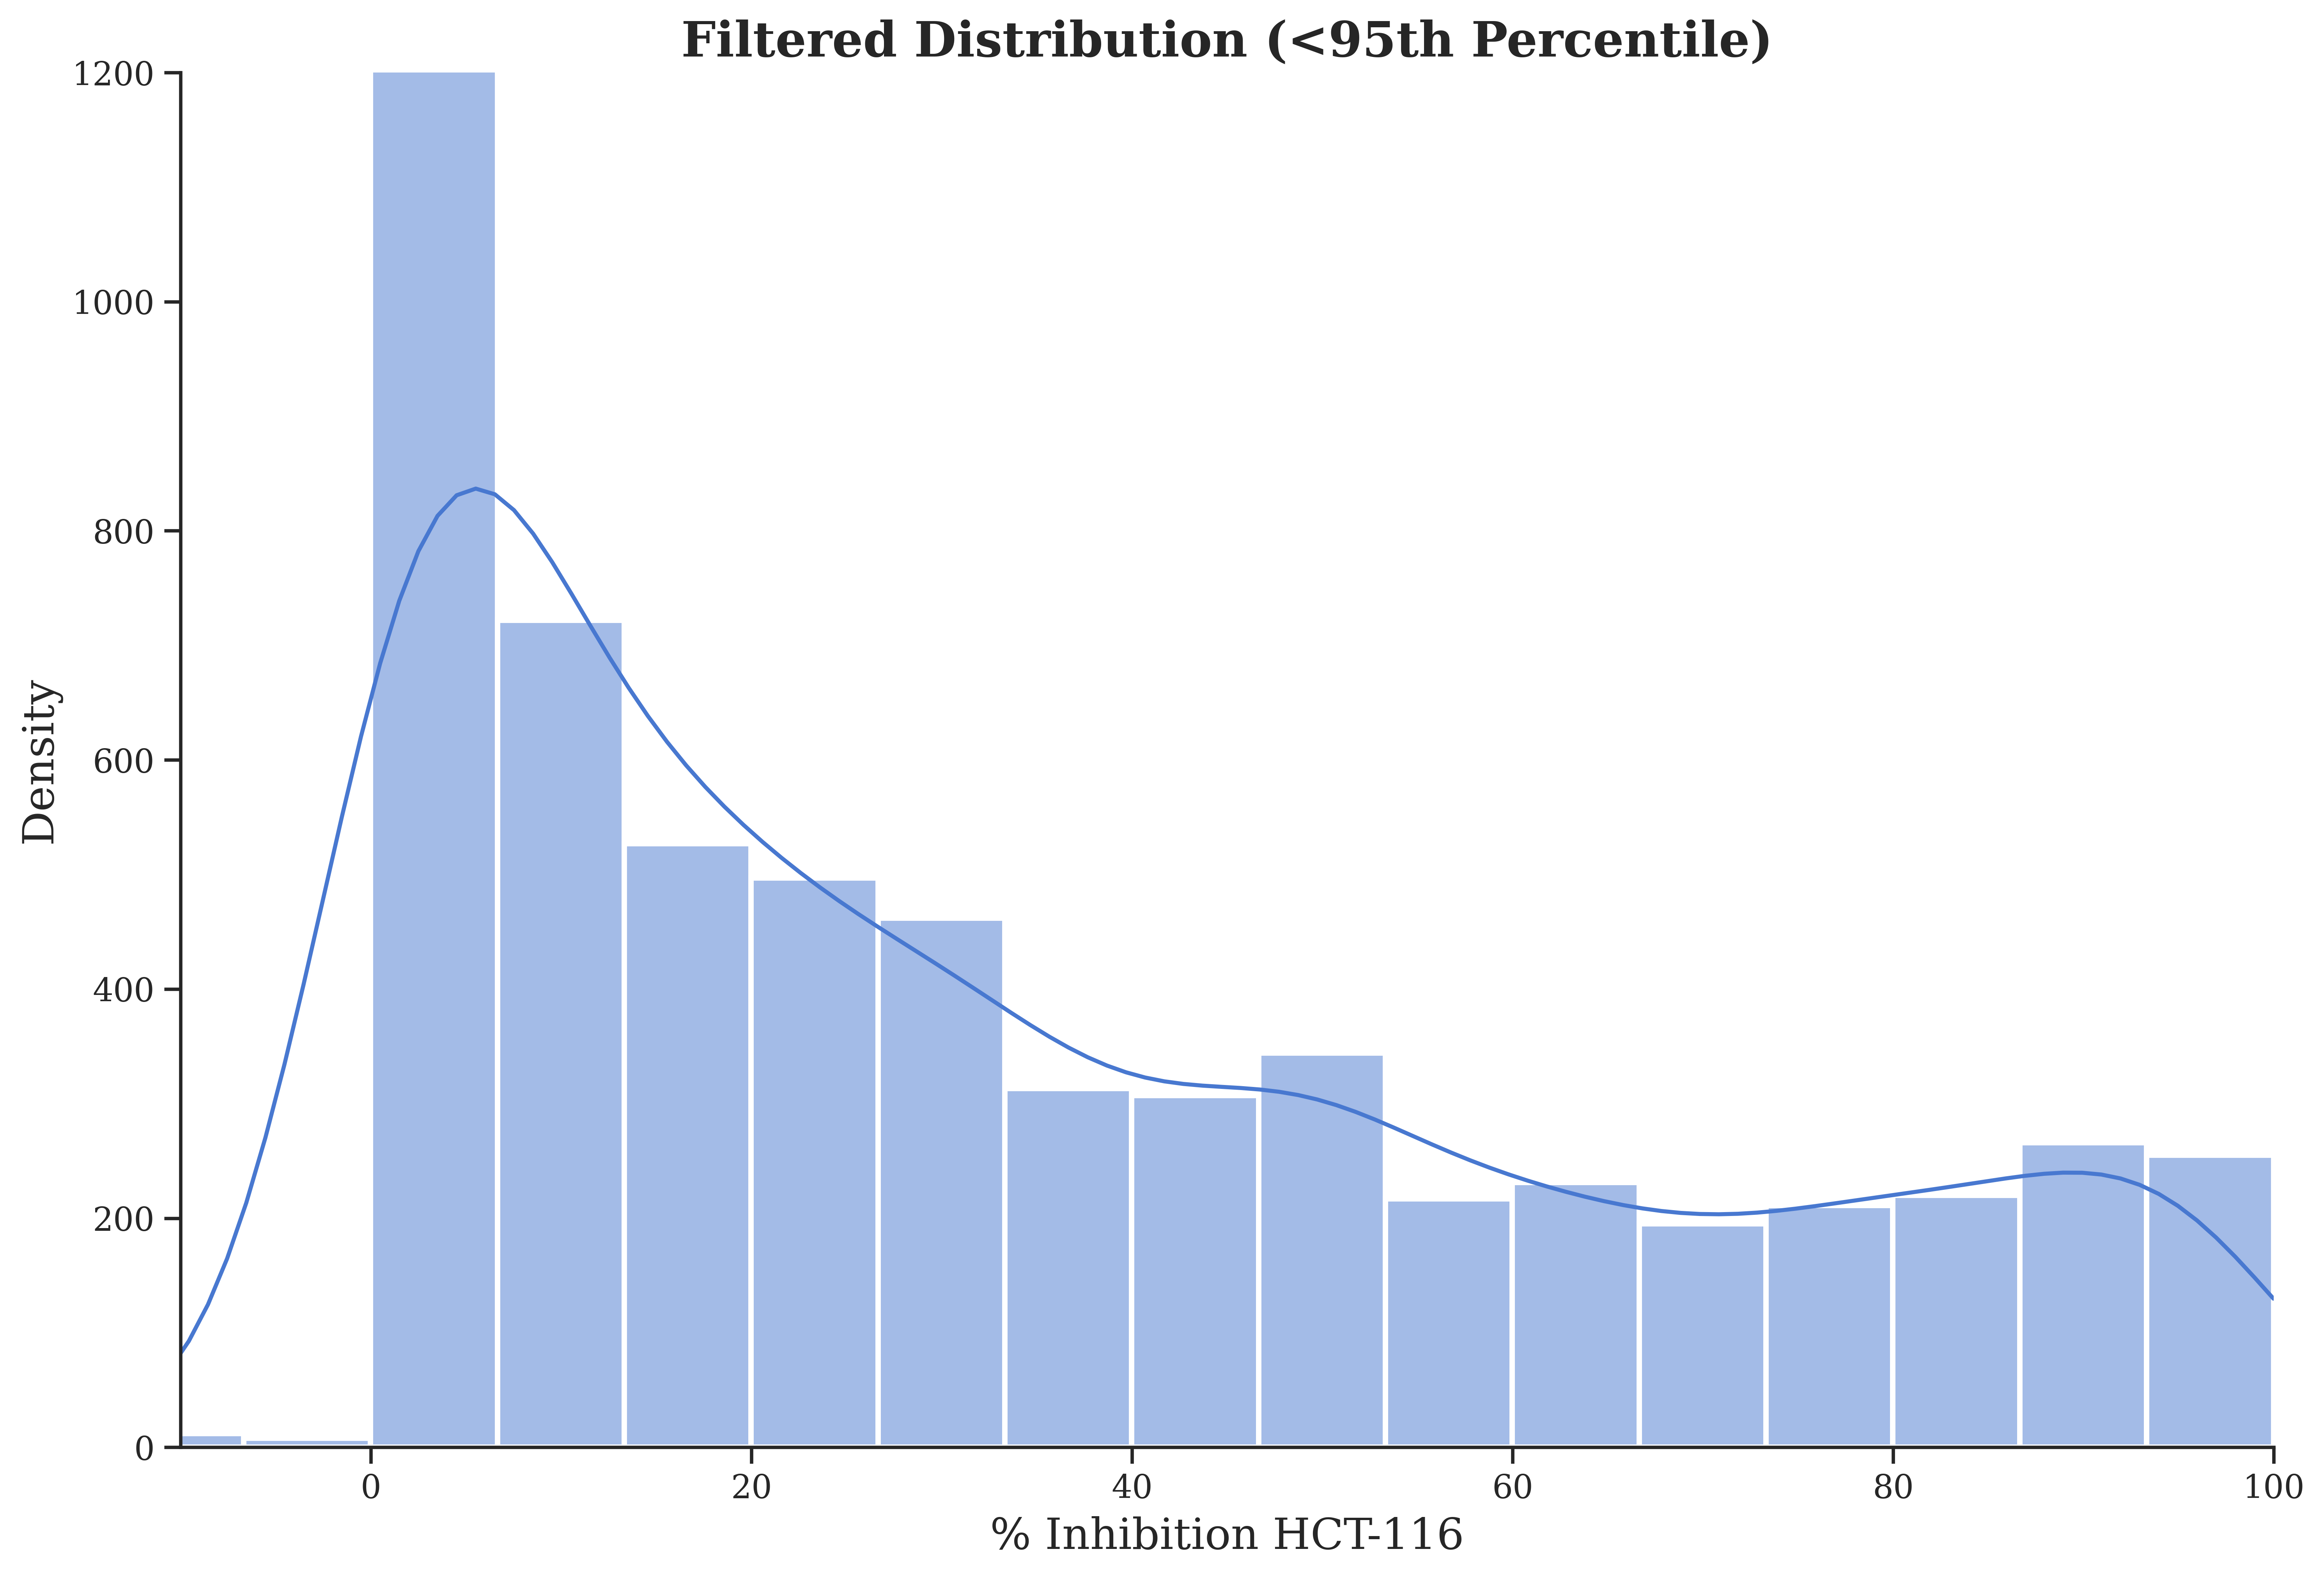
\includegraphics[width=0.8\textwidth]{cleandatadist.png}% Replace with your image filename
	\caption{Distribution of clean dataset of HCT-116}
	\label{fig:cleandist} % Optional: use \label for referencing
\end{figure}

Development of ML models are heavily dependent on the data quality \cite{zhou2024dataquality}. Erroneous and misleading predictions generated by the models are often associated with outliers that were not removed during the training and testing period. Unfiltered dataset was observed to have 70.16 skewness, indicating that most of the data outliers are located on the positive tail end of the curve. If not removed, it is expected to result in positive errors in predictive models. Thus, the dataset used in this study was pre-processed prior to modelling, resulting to filtered data that has a  skewness of 0.05386, leading to a significant improvement in distribution. \autoref{fig:cleandist} shows that filtered/clean data has an asymmetric normal distribution (i.e., imbalanced data set). SMOTE serves to balance the minority and majority class of the data set, removing positive biases in model predictions (\autoref{fig:SMOTE}).

\FloatBarrier
\begin{figure}[h]
	\centering
	\begin{minipage}{\textwidth}
		\centering
		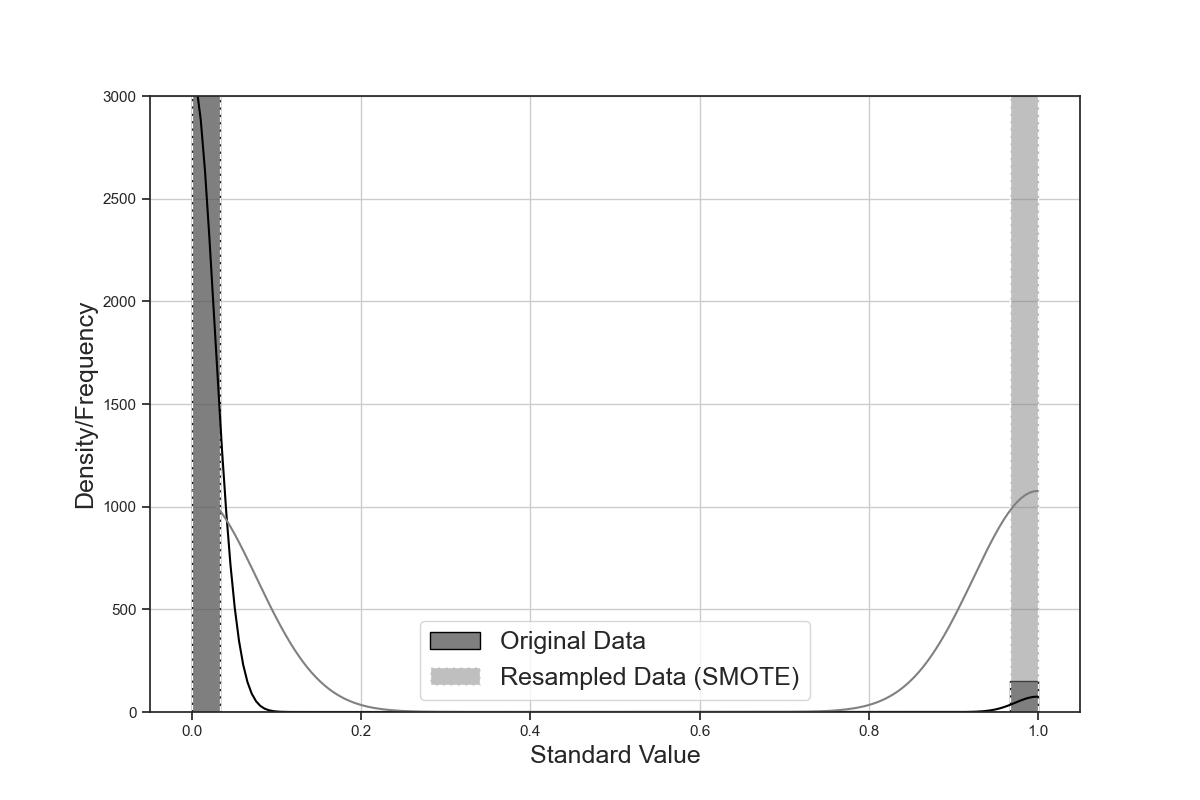
\includegraphics[width=1\textwidth]{SMOTEbw.png}
		\vspace{-1cm}
		\caption{Comparison of distributions before and after SMOTE}
		\label{fig:SMOTE}
	\end{minipage}
\end{figure}
\FloatBarrier

%\begin{figure}[htbp] % 'h' places the figure approximately here
%\centering
%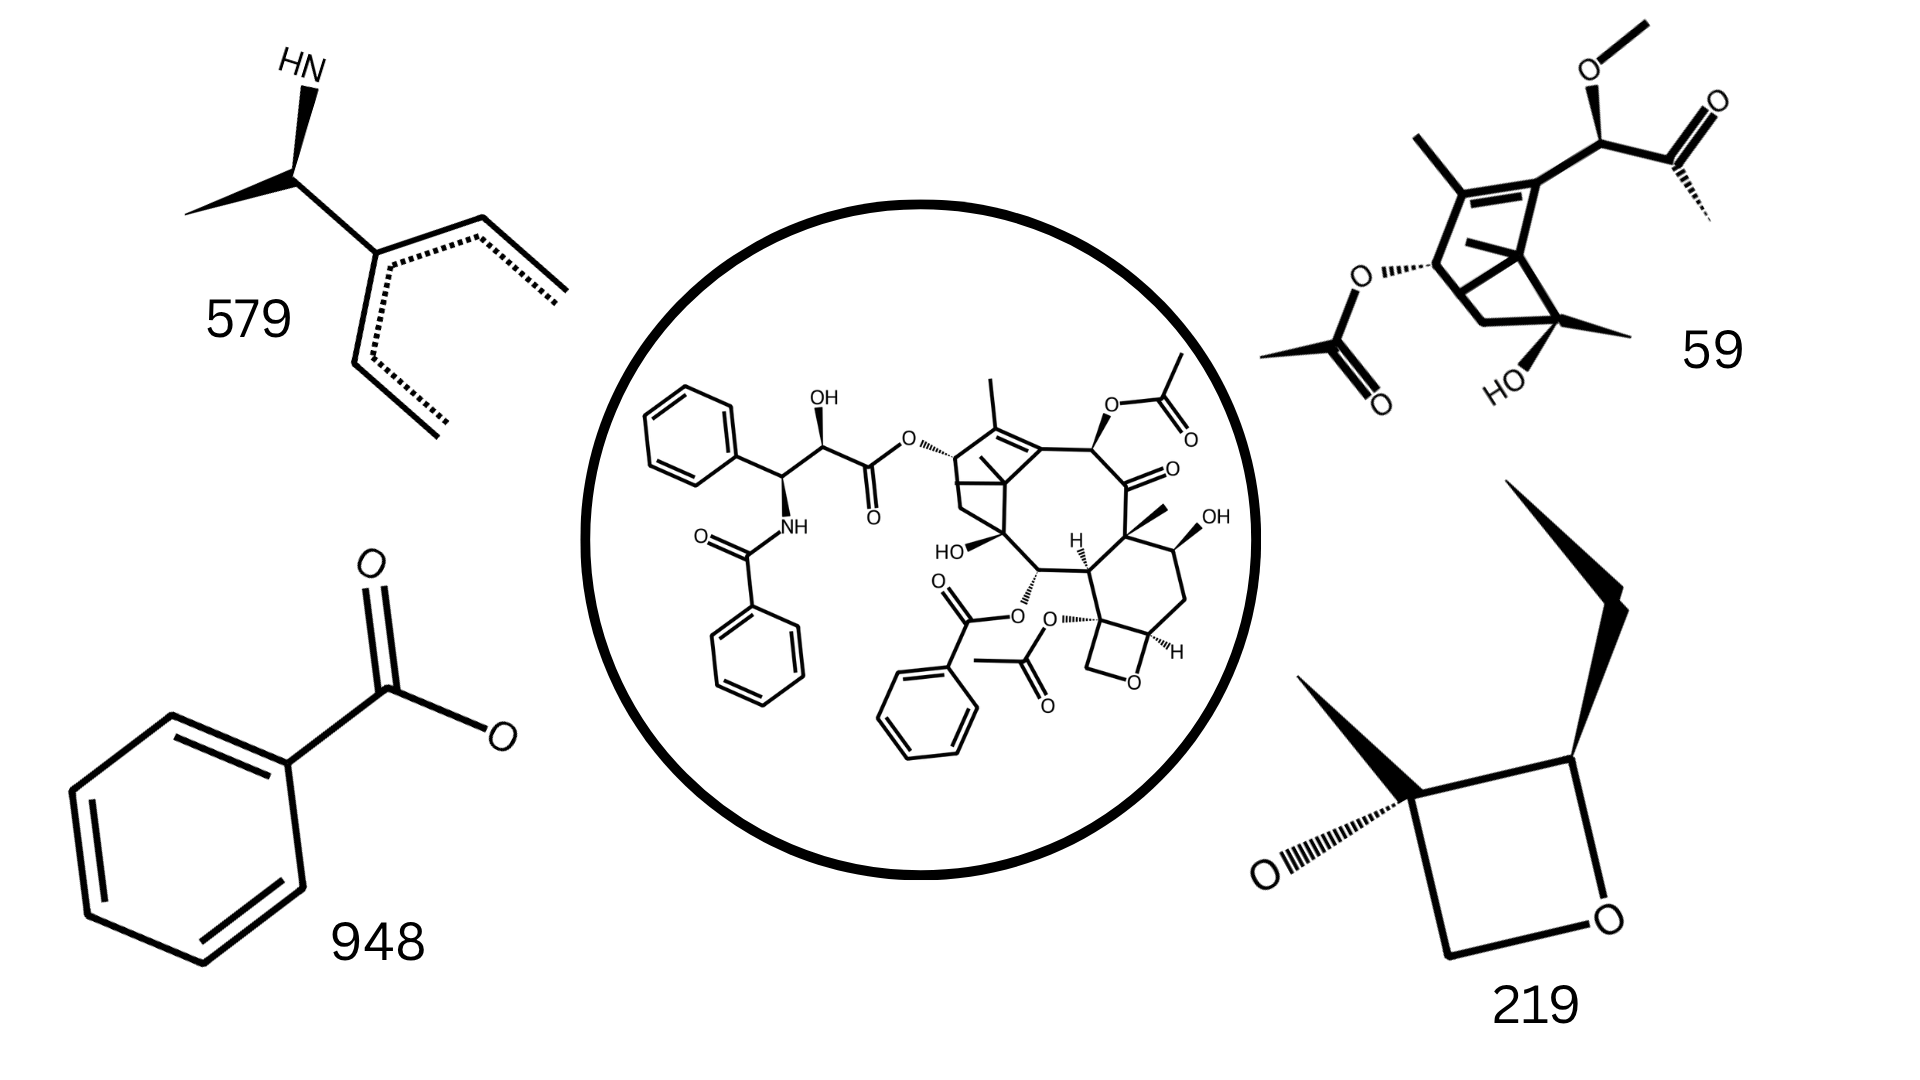
\includegraphics[width=0.7\textwidth]{fragmentation.png}% Replace with your image filename
%\caption{Fragmentation of Target Compound to Produce MF and Bit Number Assignment}
%\label{fig:mfex} % Optional: use \label for referencing
%\end{figure}

The MFA produced a maximum of 2048 bits for each compound and approximately 12 million bits in total were analyzed in this study. \autoref{tab:summary} presents the summary of pre-processing and generation of MFPs and MPs from MFA. The CBC method revealed that there are bits that were frequently present in molecules with or without bioactivity against HCT-116. \autoref{fig:top10crudebits} shows the top 10 bits observed through CBC. Nearly all of the top 10 bits identified from CBC can be considered as small fragments. Changes in these bits could lead to positive or negative effects to bioactivity (\autoref{fig:top10crudebits}). Since the bits were not segregated and non-significant bits were not removed prior to bit frequency counting, it is possible that the identified top 10 bits represents a mixture of positive, negative and non-significant bits. 
%To perform QSAR studies of the given clean data set, the generation of MF's plays the pivotal role on giving the MFA its capacity to perceived structural patterns in a binary format.  

%To gain a meaningful structural insight, the CBC and CSBC were employed. In essence, the presence and absence of particular bits and its relation to \% Inhibition can be simply detected by means of counting its frequency. This simple logic was leveraged in CBC method, wherein after the generation of MP's and MF's of the compounds, bit of a specific MF's were counted and ranked (see \autoref{tab:t10crude}). Essentially, the MF with highest bit frequency were expected to have a relationship with the \% Inhibition of compounds against HCT-116. On selecting the top 10 bits, researchers set the frequency values to at least 50\% of the total data, assuming that it is equal to the amount of observation that has a significance.

\begin{table}[h] % Optional: for floating the table
	\centering
	\begin{threeparttable}
		\renewcommand{\arraystretch}{1.2} % Adjust row spacing (1.2x normal)
		\small
		\begin{tabular}{p{3cm} p{4cm} p{4cm} p{2cm} p{2cm}} % Five columns (all centered and with vertical borders)
			\hline
			Molecule ChEMBL ID & SMILES & Mols \tnote{a} & \%Inhibition & MP \\ 
			\hline
			CHEMBL259084 & O=C(O)c1ccc$\ldots$ & rdkit.Chem.rdchem.Mol object at 0x00000225A15$\ldots$ & 6.400 & 111010101$\ldots$ \\ 
			CHEMBL224940 & CCCCN1CCN(C(=O)$\ldots$& rdkit.Chem.rdchem.Mol object at 0x00000225A15$\ldots$ & 27.000 & 101110100$\ldots$ \\ 
			CHEMBL2029910 & CN1CCN(C(=O)c2cc$\ldots$ & rdkit.Chem.rdchem.Mol object at 0x00000225A15$\ldots$ & 0.003 & 101010100$\ldots$ \\ 
			\vdots & \vdots & \vdots & \vdots & \vdots \\
			CHEMBL3813873	 & FC(F)(F)c1ccc$\ldots$ & rdkit.Chem.rdchem.Mol object at 0x00000225A16$\ldots$ & 4.280 & 111110101$\ldots$ \\ 
			\hline
		\end{tabular}
		\begin{tablenotes}
			\item[a] Mols indicates molecular object data type which is interpreted as a display or png file by the rdkit package. 
		\end{tablenotes}
	\end{threeparttable}
	\caption{Summary of data profiles for compounds}
	\label{tab:summary}
\end{table}

\begin{figure}[htbp!] % 'h' places the figure approximately here
	\centering
	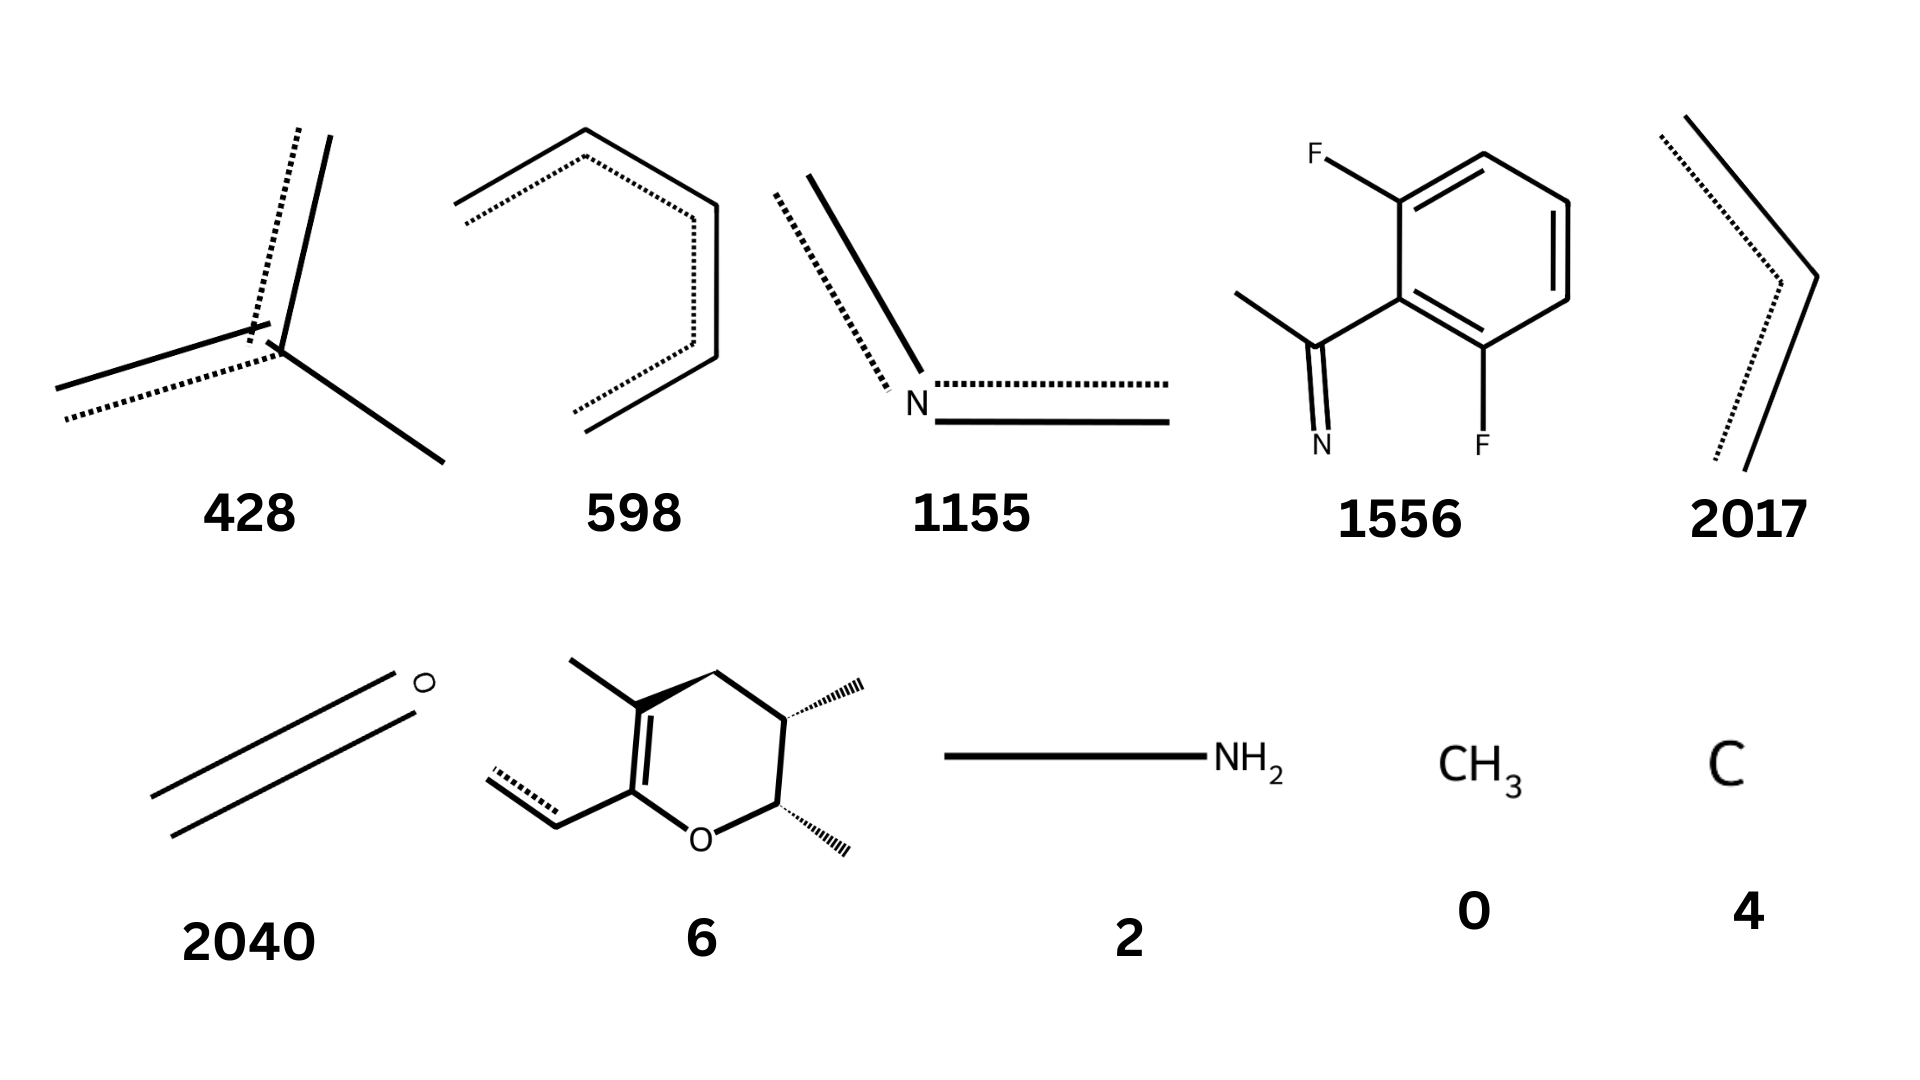
\includegraphics[scale=0.30]{top10crudebitsv2.png} % Replace with your image filename
	\caption{CBC top 10 bits: 2D - structures}
	\label{fig:top10crudebits} % Optional: use \label for referencing
\end{figure}

%Based on the results CBC identified the following bits: 0, 2, 4, 2017, 2040, 428, 6, 1556, 1155, and 598 as significant bits. Wherein, the algorithm suggest that these bits have a significant relationship with the bioacitivity of compounds. The machine 2D perception of the bits are quite unique, for it accounts the following: a) central atom (colored with blue dots); b) atomic substitution (color yellow)\footnote{yellow color represents sulfur substitution or other electronegative atoms}; and c) predicted bonds at the end of structure (colored with gray)\footnote{dashed grey line represents partial bonds}. Structurally, almost all of them were considered to be a small fragments, this could mean that structural or conformational changes in this bits could lead to inactivity of a compound (\autoref{fig:top10crudebits}). However, it was assumed that since the bits were not segregated and non-significant bits are not removed prior to bit frequency counting, probably the constituents of Top 10 bits from CBC could have a mixture of positive, negative and non-significant bits. To verify this assumption, the identified structural features will be used in the creation of CBC-ML, wherein the machine will be train and test to classify compounds activity based on the input features extracted from this method.  

The CBC method is a simple technique to identify the significant bits from the clean dataset, but it does necessarily incorporate information on the position and neighboring structural motifs. Therefore, there may be cases that the presence or absence of a particular bit will have different meanings depending on their position or structural environment. In contrast, because CSBC employed blind clustering, it allows for the categorization of data prior to counting. This intermediate step gives an insight on the different clusters that exist in the given dataset, which could lead to classification and discovery of new structural patterns. One underlying assumption in the application of CSBC is that common features shared among clusters will implicitly incorporate the dependence on position and neighborhood of structural motifs. Furthermore, subtraction of clusters  may naturally remove non-significant bits which could lead to more efficient identification of positively and negatively contributing bits. 

%several critical factors to understand and accurately classify the compounds based on their structural features. The researchers identified these critical factors to be the position and neighbor of bits. The algorithm used in CBC does not take into account where does the bits located and what are its neighbors during the counting process. Therefore, it is probable that there will be cases that the presence or absence of a particular bit will have different meanings depending on their position or neighbor. To mitigate this possibility, another method is developed to account these kind of scenarios which is called CSBC. In CSBC, blind clustering was first employed prior to counting, this was done to segregate the data sets and simplify it prior to counting. This intermediate step gives an insight about the different clusters that exist in the given data set that could lead to classification and discovery of new structural patterns. Essentially, the researchers assumed that, these clusters of compounds will have something in common and different, therefore, if these information could be extracted, probably the dependency in position and neighbors of the compounds could be understood. Furthermore, researchers also assumed that by doing blind clustering the presence of non-significant bits could be removed giving a way to identify early on the positive and negative bits. 

Result shows that the optimum number of clusters for the given data set using the Elbow Method is 5. K-Clustering divided 6304 \% Inhibition data into 5 categories which were classified as: a) HI (purple); b) MI (blue); c) LI (orange); d) VLI (green); and e) NI (red) (\autoref{fig:cluster}). The VLI region in contains the compounds with \% Inhibition of around -20 to 20, and it can be considered as the neutral point of the bioactivity \footnote{region of the dataset that could be regarded as having non-significant bioactivity or close to 0 \% Inhibition} (\autoref{fig:cluster}). The structural features of compounds under this category may considered to be non-significant and must be removed. In addition, it is also assumed that from the set neutral point going up and down to HI and NI respectively may mean that alteration of molecular structures in these regions might lead to maximization or minimization of bioacitivity against HCT-116. Therefore, subtraction of molecular MPs in the VLI region from those in the HI, MI, LI, and NI regions may lead to the extraction of structures that either increase or decrease their bioactivity.        

%\begin{figure}[h] % 'h' places the figure approximately here
	%\centering
	%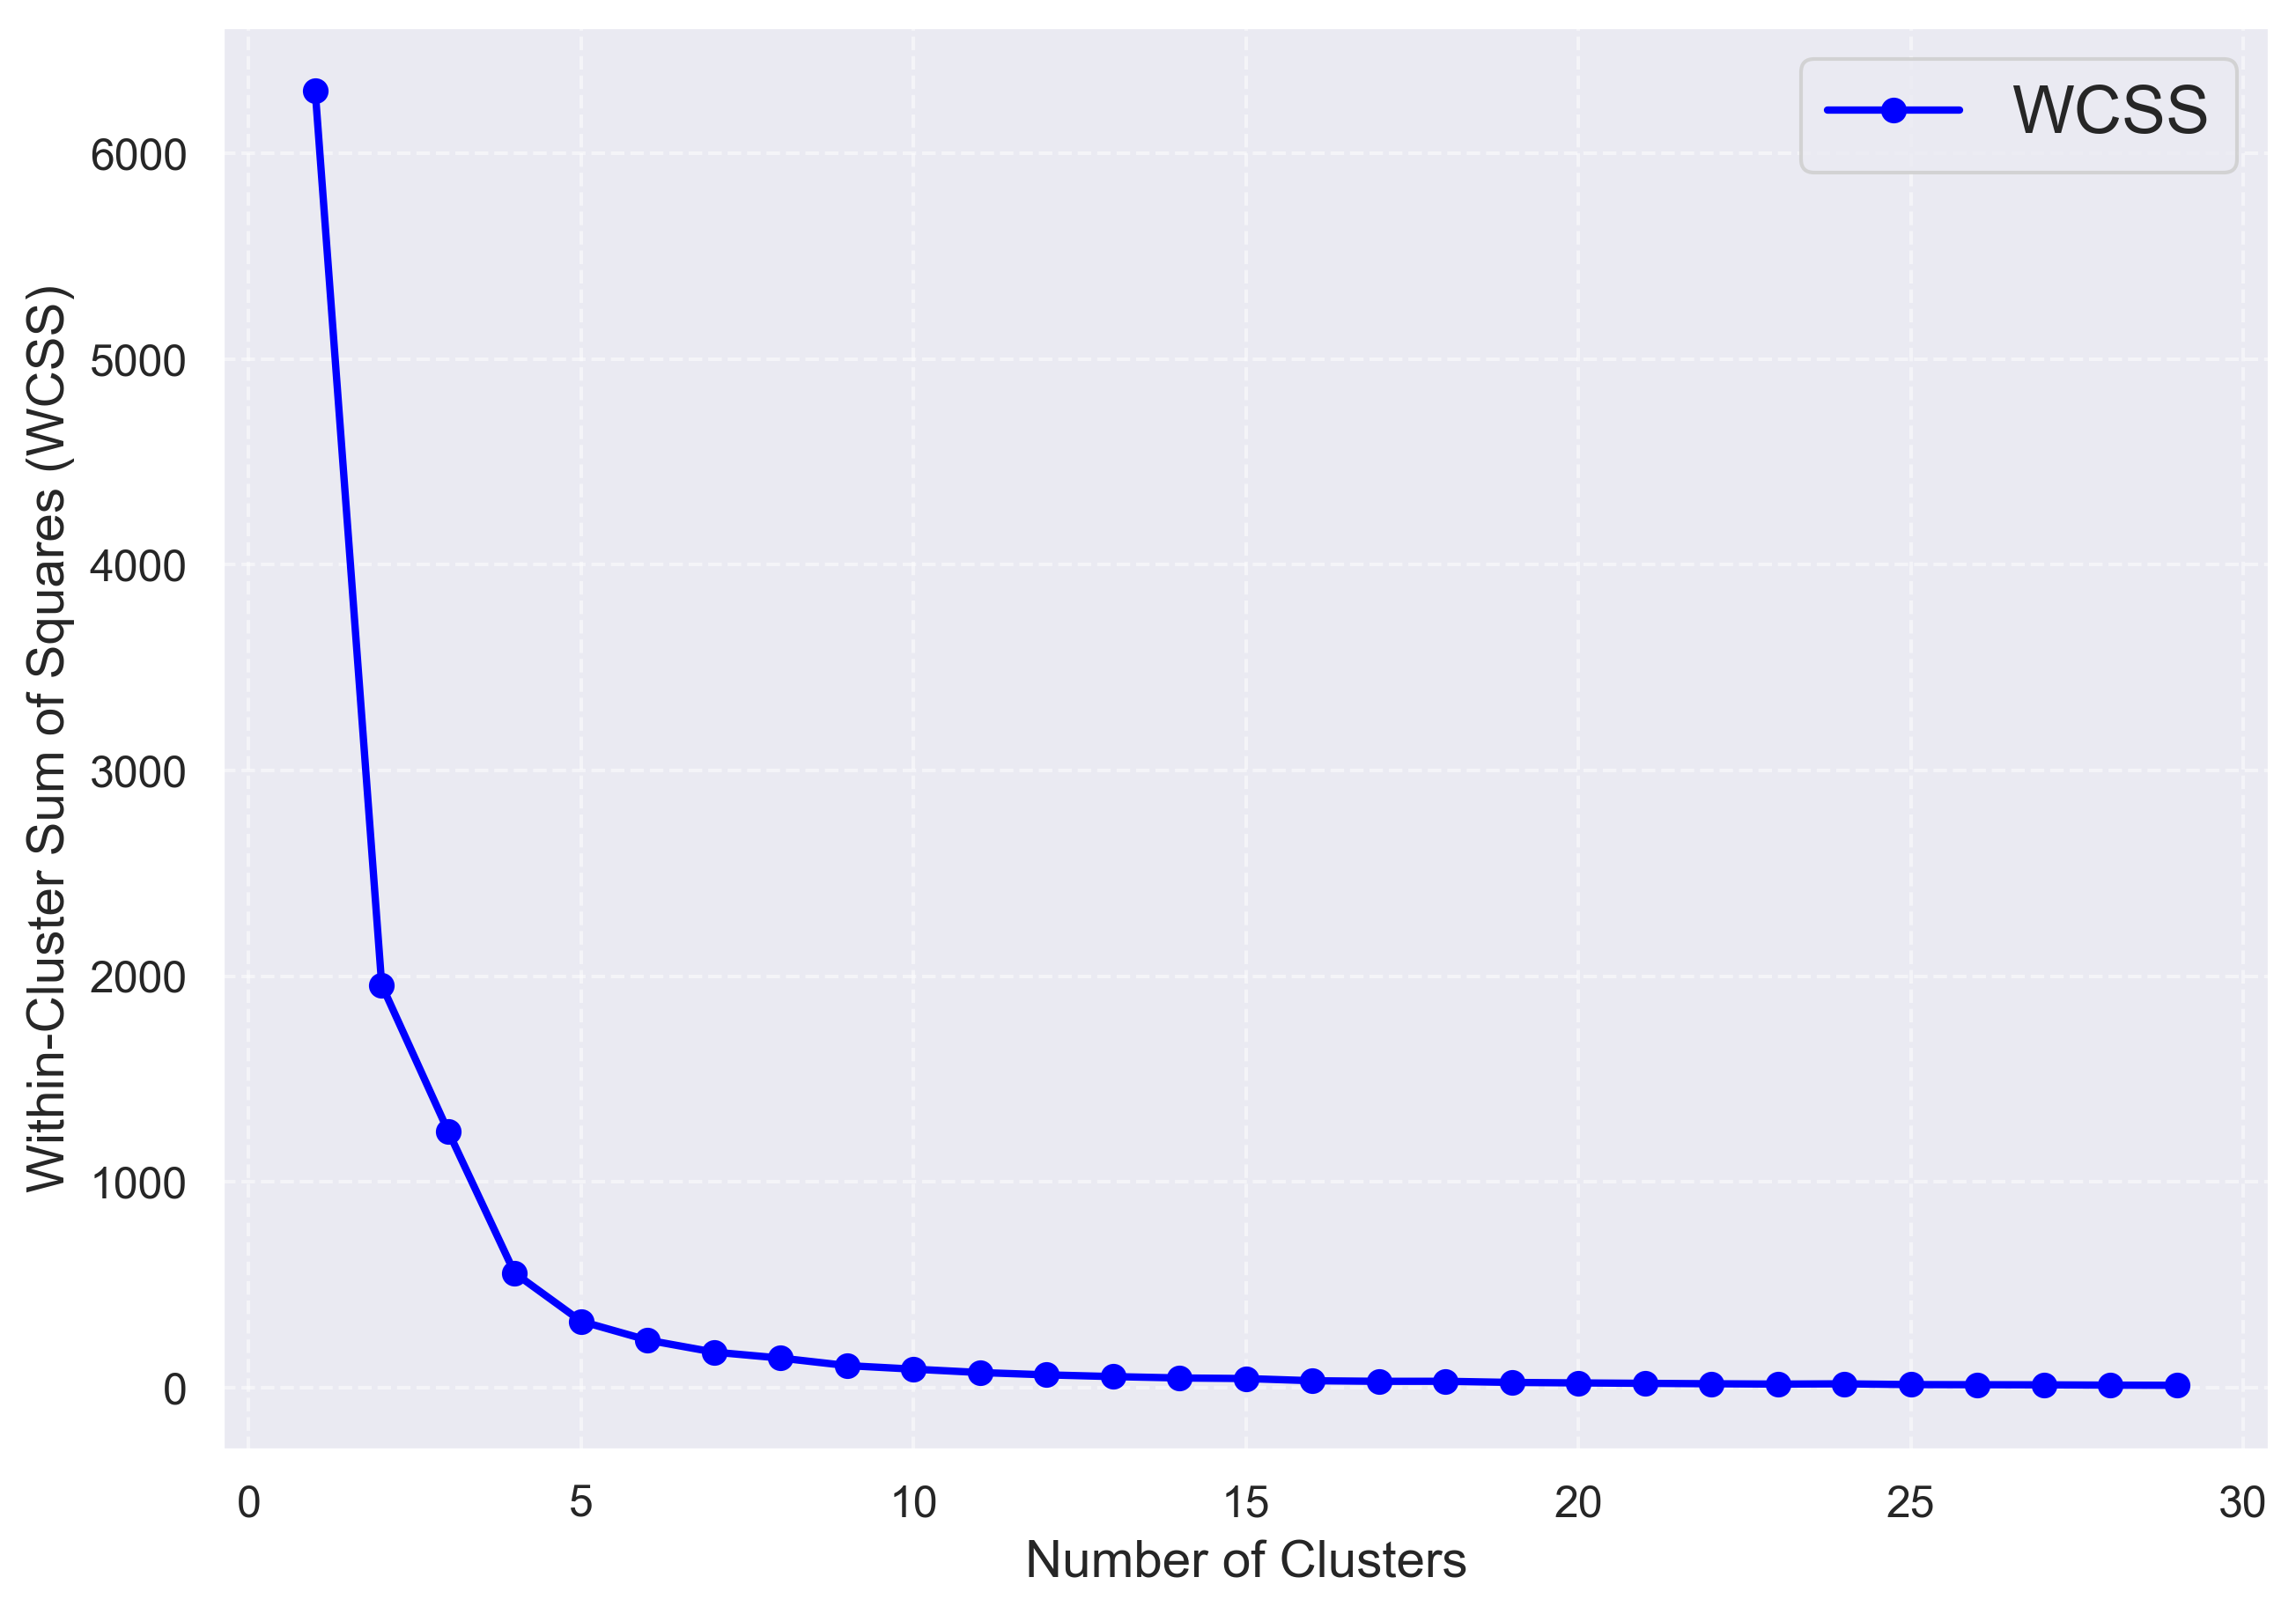
\includegraphics[width= 0.9\textwidth]{elbow.png} % Replace with your image filename
	%\caption{Elbow Method for Optimal Number of Clusters}
	%\label{fig:elbow} % Optional: use \label for referencing
%\end{figure}


\begin{figure}[h] % 'h' places the figure approximately here
	\centering
	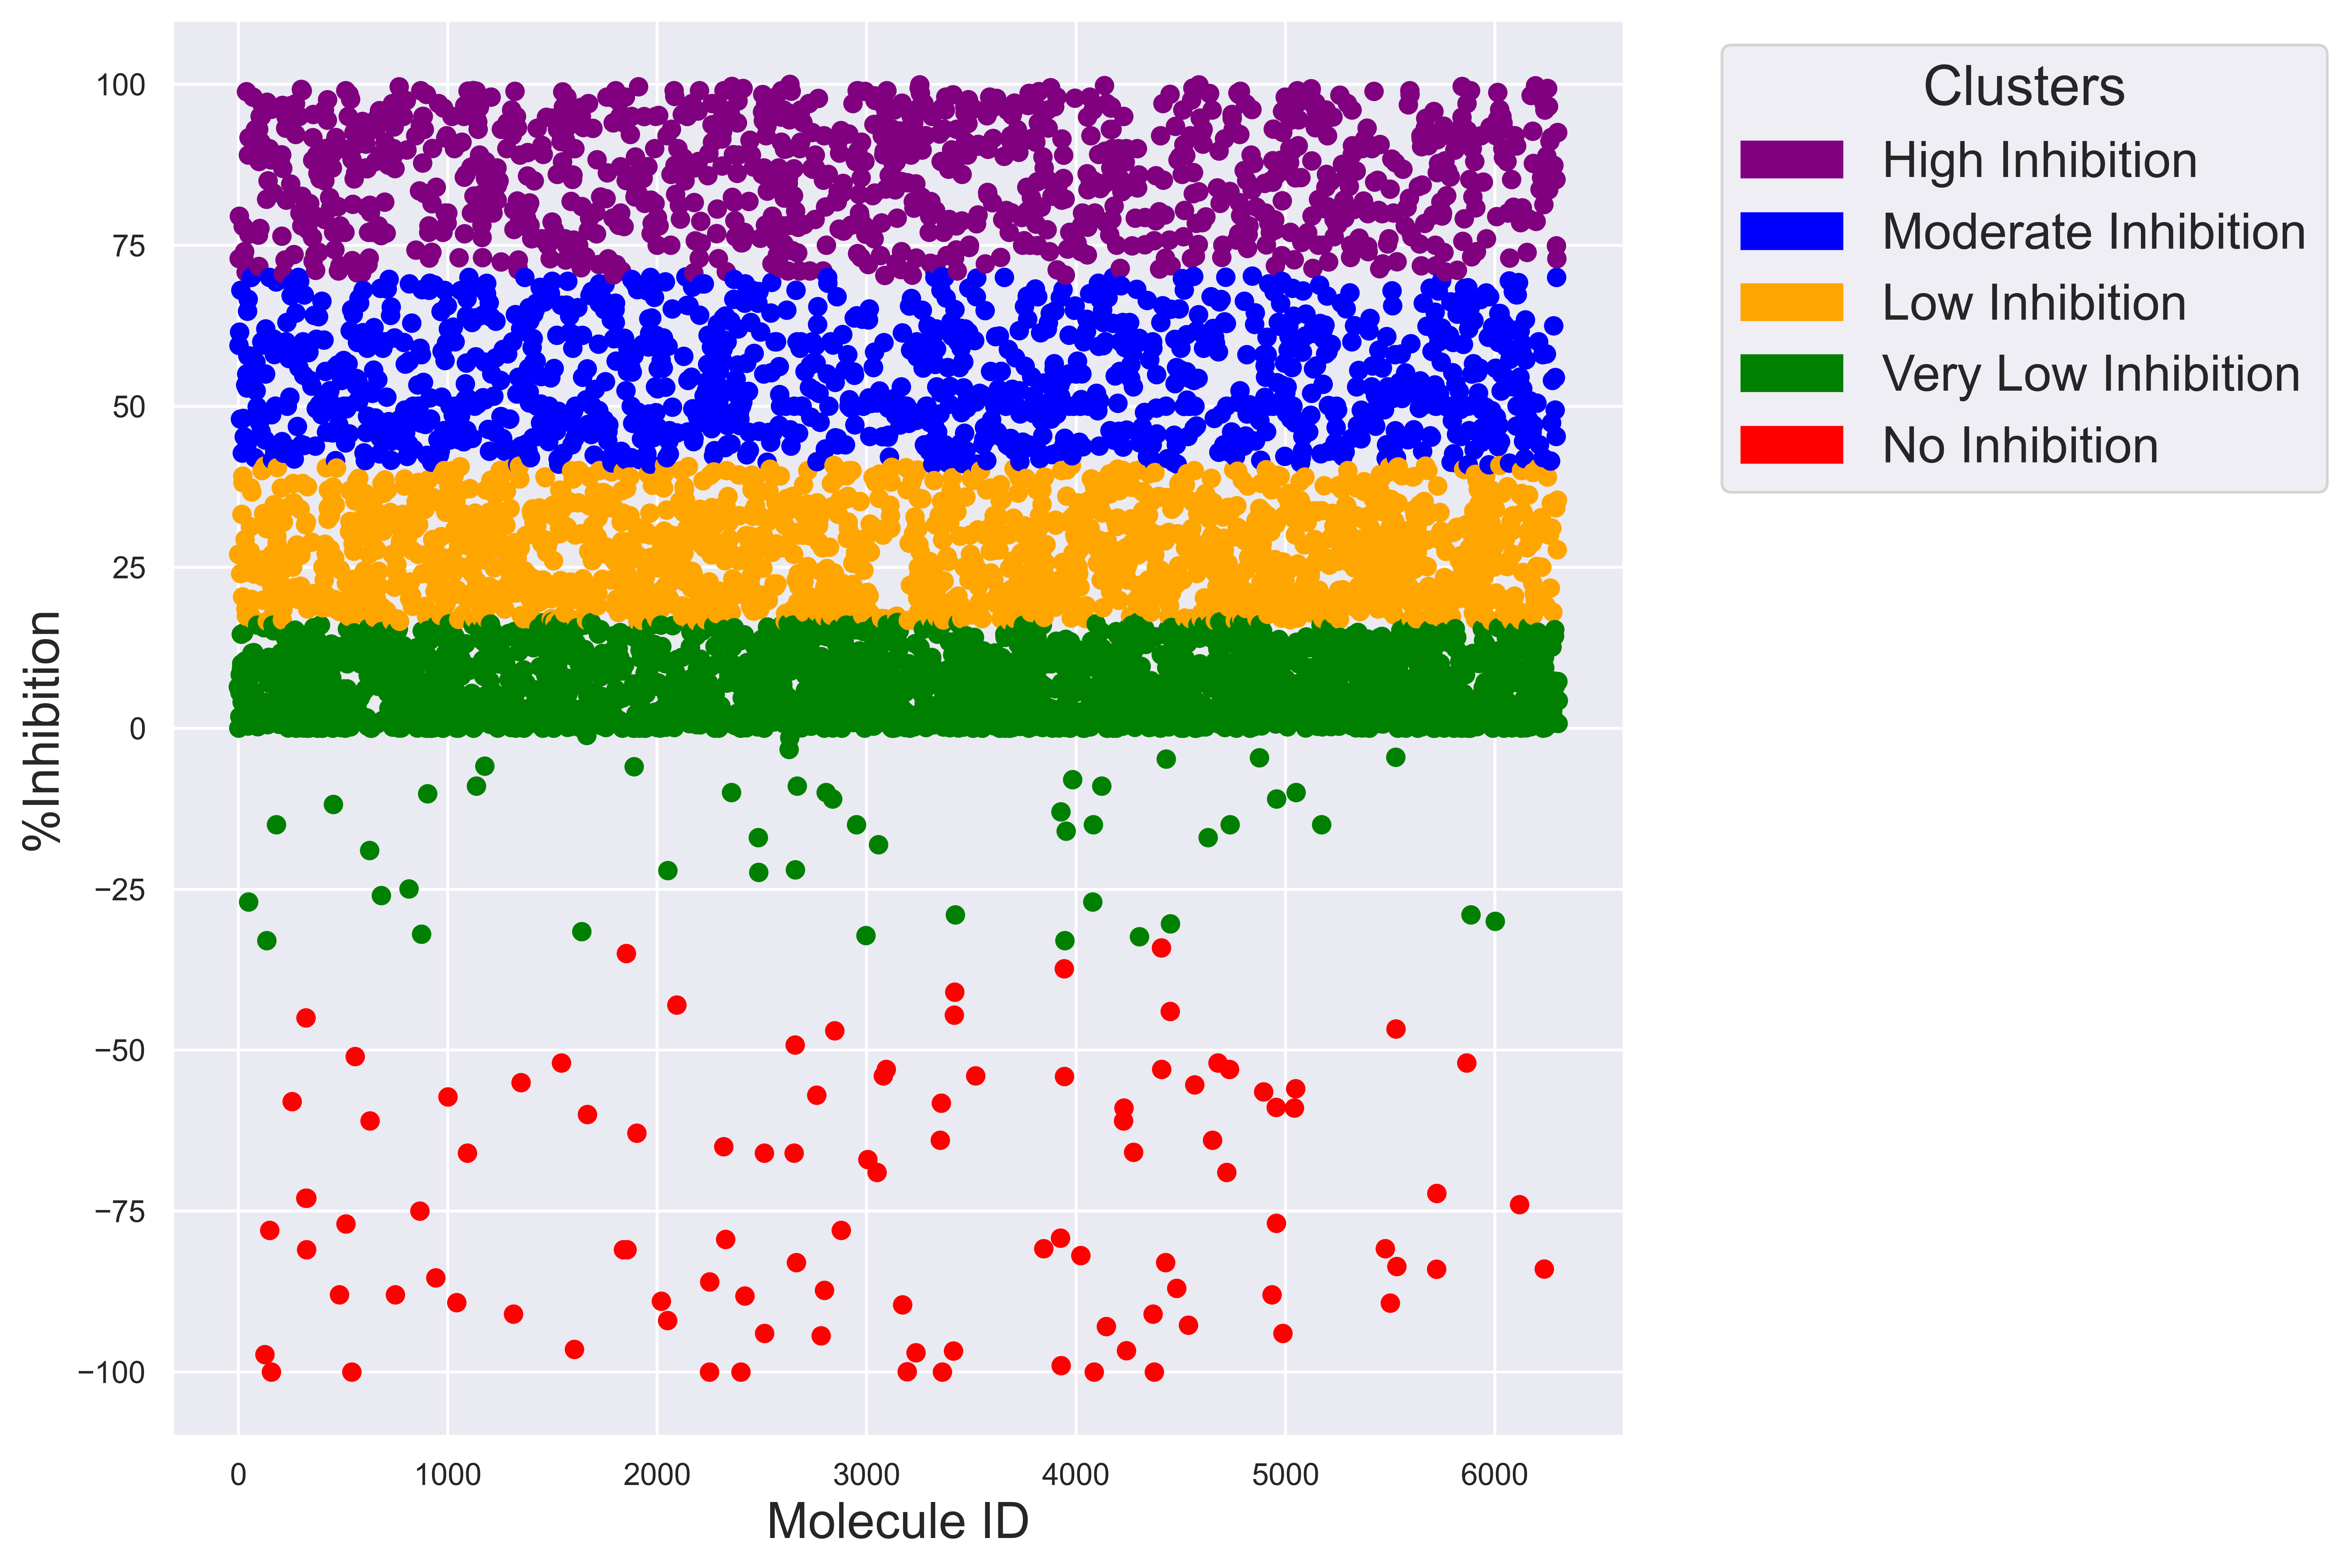
\includegraphics[scale=0.6]{cluster.png} % Replace with your image filename
	\caption{Cluster analysis of bioactivity against HCT-116}
	\label{fig:cluster} % Optional: use \label for referencing
\end{figure}

HI, MI, LI, VLI and NI have the matrix dimensions of (1035 x 2048), (1162 x 2048), (1588 x 2048), (2417 x 2048), and (102 x 2048) respectively. The entire process of VLI subtraction to all categories results to a total of 9,394,879 newly formed MPs removing approximately 3,515,713 non-significant MFs. These new MPs that essentially contain the PBs and NBs were simplified by means of combining similar MPs and counting their frequencies. From this process, the PBs and NBs were identified based on their relationship with \% Inhibition against HCT-116, ranked based on frequency, and compared to identify commonalities. The summary of top bits is shown in \autoref{fig:mostcombits}. It must be noted that the resulting difference between VLI-HI and VLI-NI were considered to be positive and negative bits. Whereas, the results from VLI-MI and VLI-LI differences were considered to be moderate bits. In addition, it was observed that there were common bits among the results within differences. It is then a matter of investigating these common bits to verify whether there is a considerable degree of retention on position and neighborhood dependency.

%These findings could imply that there could be a position or neighbor dependency among the observed bits, which probably explains its presence among all the clusters.


%mentioned bits were observed on the compounds with high, moderate, low, and negative bioactivity against HCT-116. Hence, it implies that these bits could be position or neighbor dependent. This implication explains why these bits were present on the compounds with high, moderate, low and negative bioactivity. These implications can be verified through the development of CSBC-ML, wherein the input features to be used are the bits generated from CSBC.


Most of the common bits were found to correspond to small molecular fragments. A close inspection of these bits offer some interesting observations. For instance, bit 857 and 428, are mirror images of each other, and are non-superimposable, reavealing that they are enantiomers. In addition, bits (1155, 2039), (1863, 1917) are constitutional and functional isomers. This small detail of change in conformation, connectivity and functional groups where detected through the use of CSBC method (\autoref{fig:mostcombits}). Hence, it is expected that it will have different weights when used in CSBC-ML. 
%Observing the structures of bits 857 and 428, notice they are mirror images of each other,however,they are non-superimposable, hence they are enantiomers. In addition, bits (1155, 2039), (1863, 1917) are constitutional and functional isomers.This small detail of change in conformation, connectivity and functional groups where detected through the use of CSBC method. Therefore, when these structural features are use in the model of CSBC-ML, it is expected to have different weights.      
%\FloatBarrier
%\begin{figure}[h]
	%\centering
	%\begin{minipage}{\textwidth}
		%\centering
		%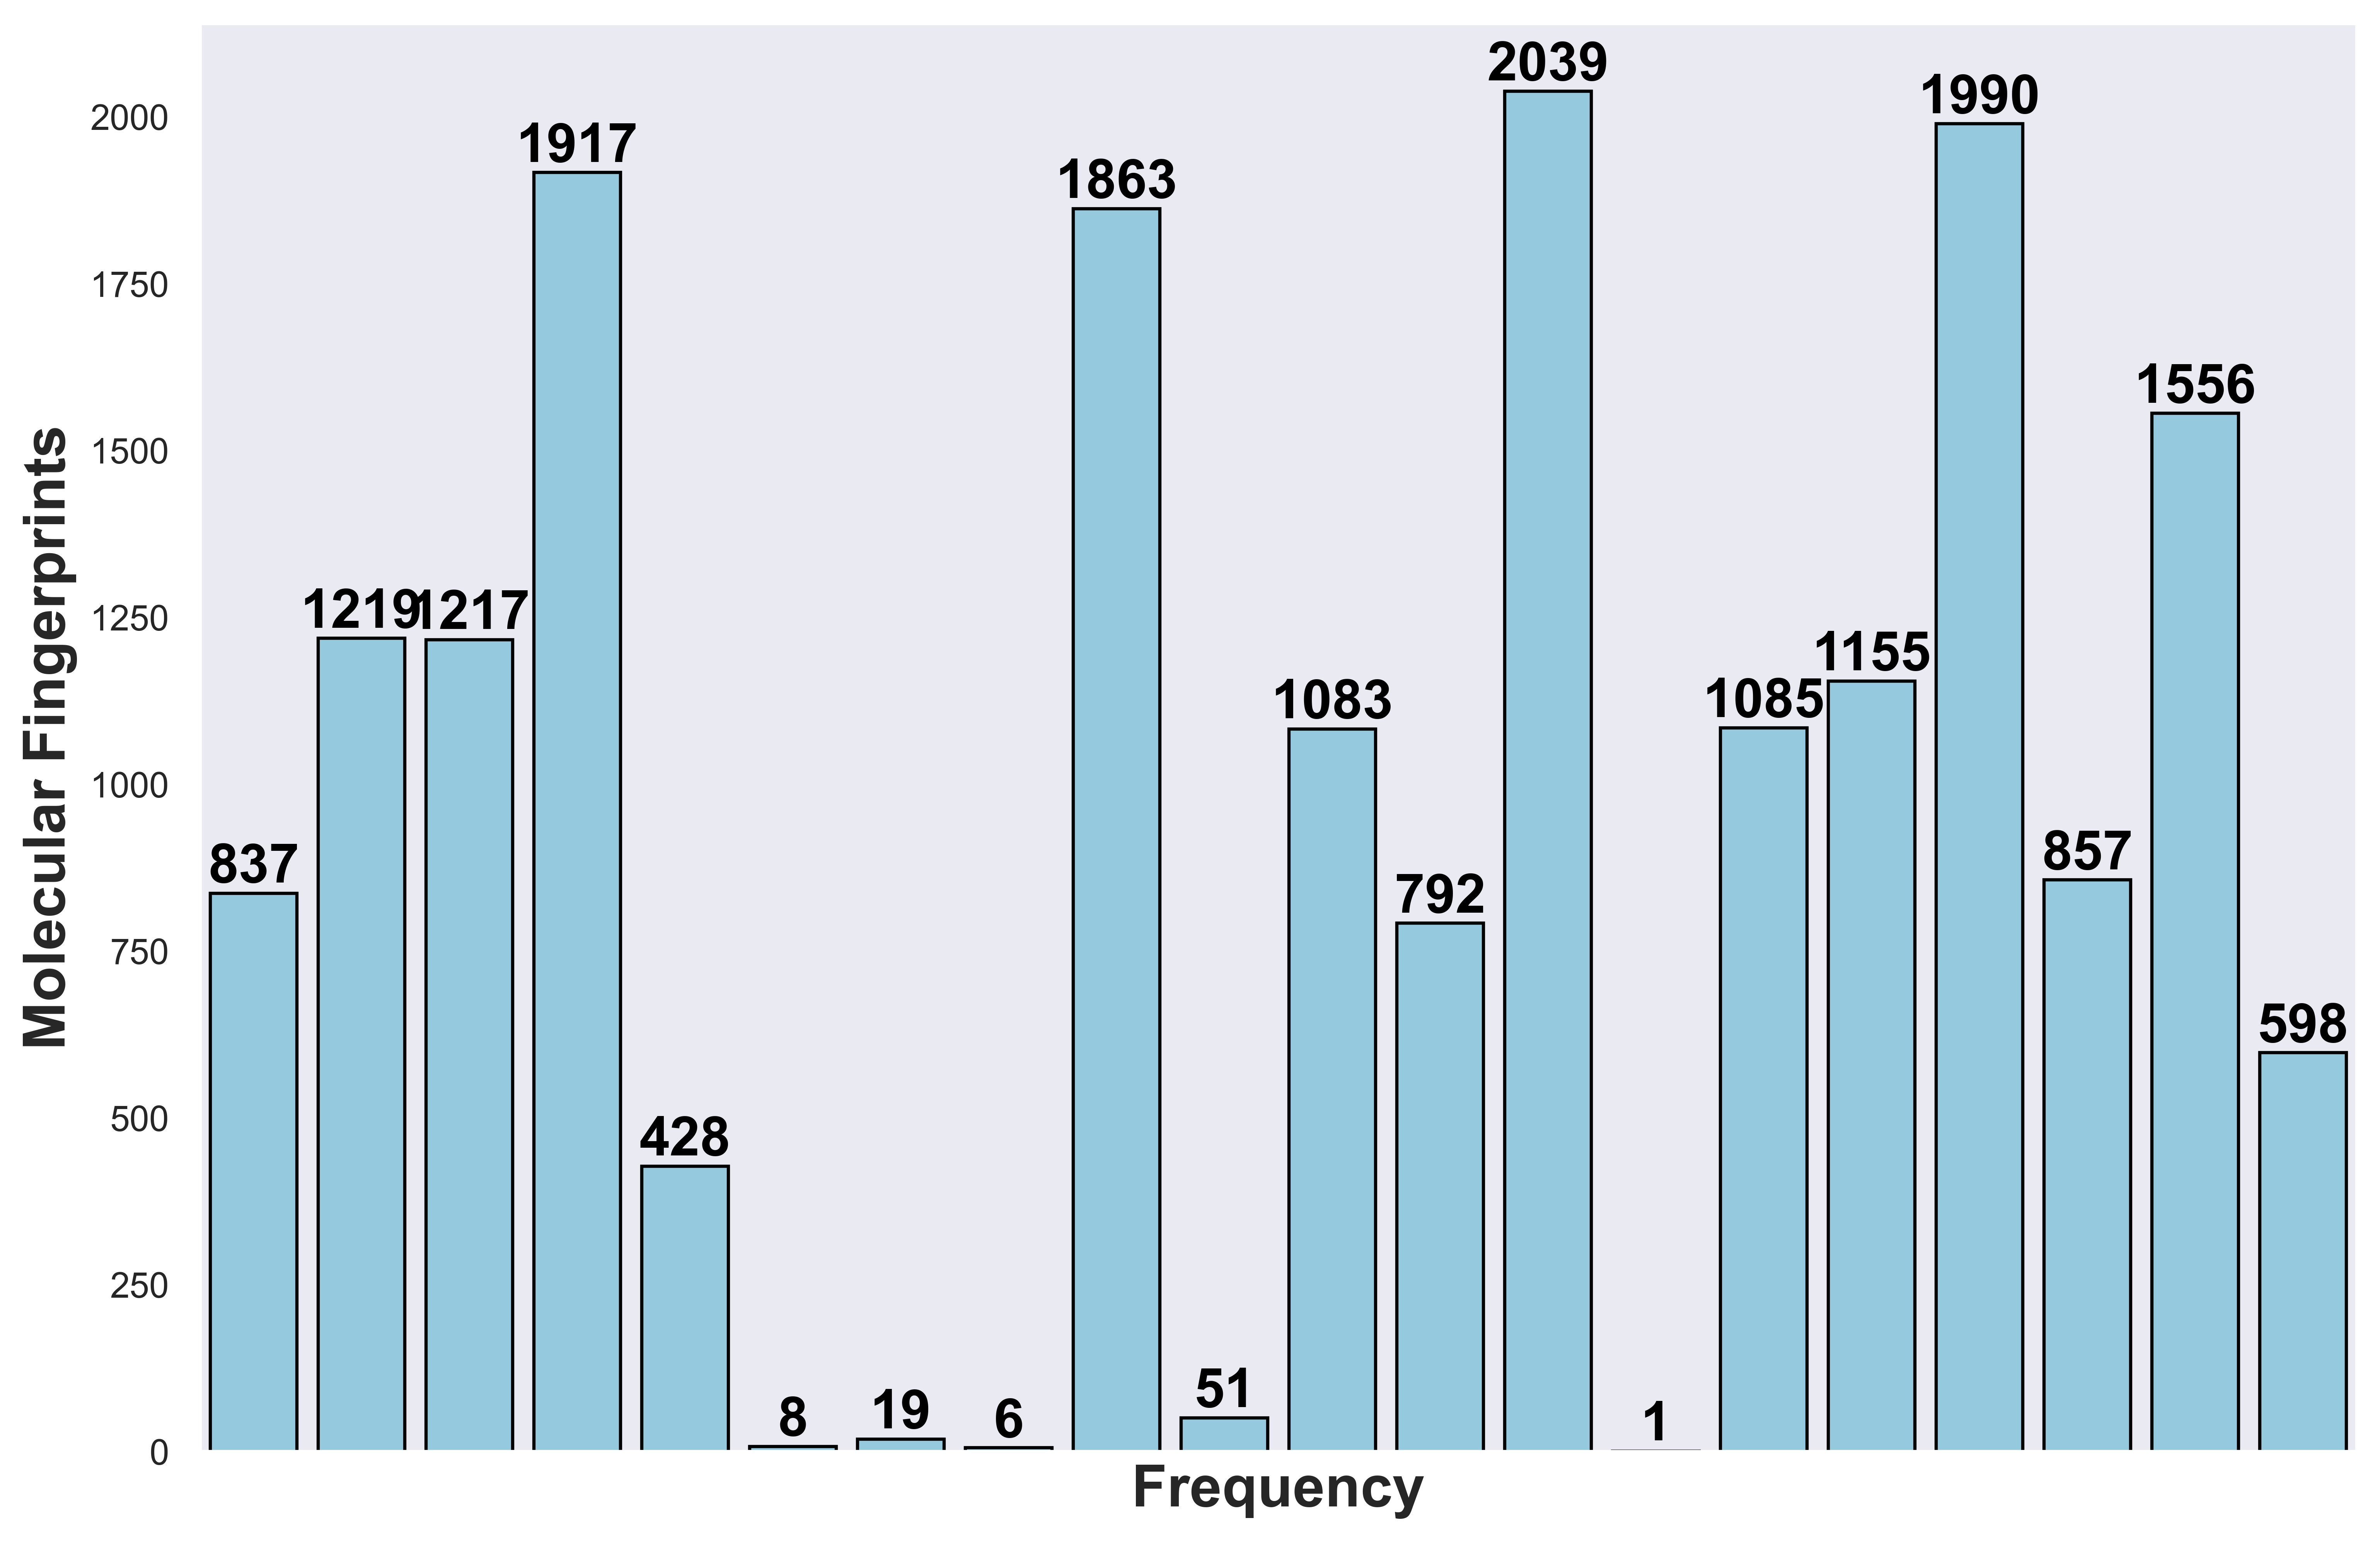
\includegraphics[width=0.8\textwidth]{bit_freq_chart.png}
		%\caption{Frequently Observed Bits in different Clusters}
		%\label{fig:most_common_bits}
	%\end{minipage}
%\end{figure}
%\FloatBarrier
\begin{figure}[h]
	\centering
	\begin{minipage}{\textwidth}
		\centering
		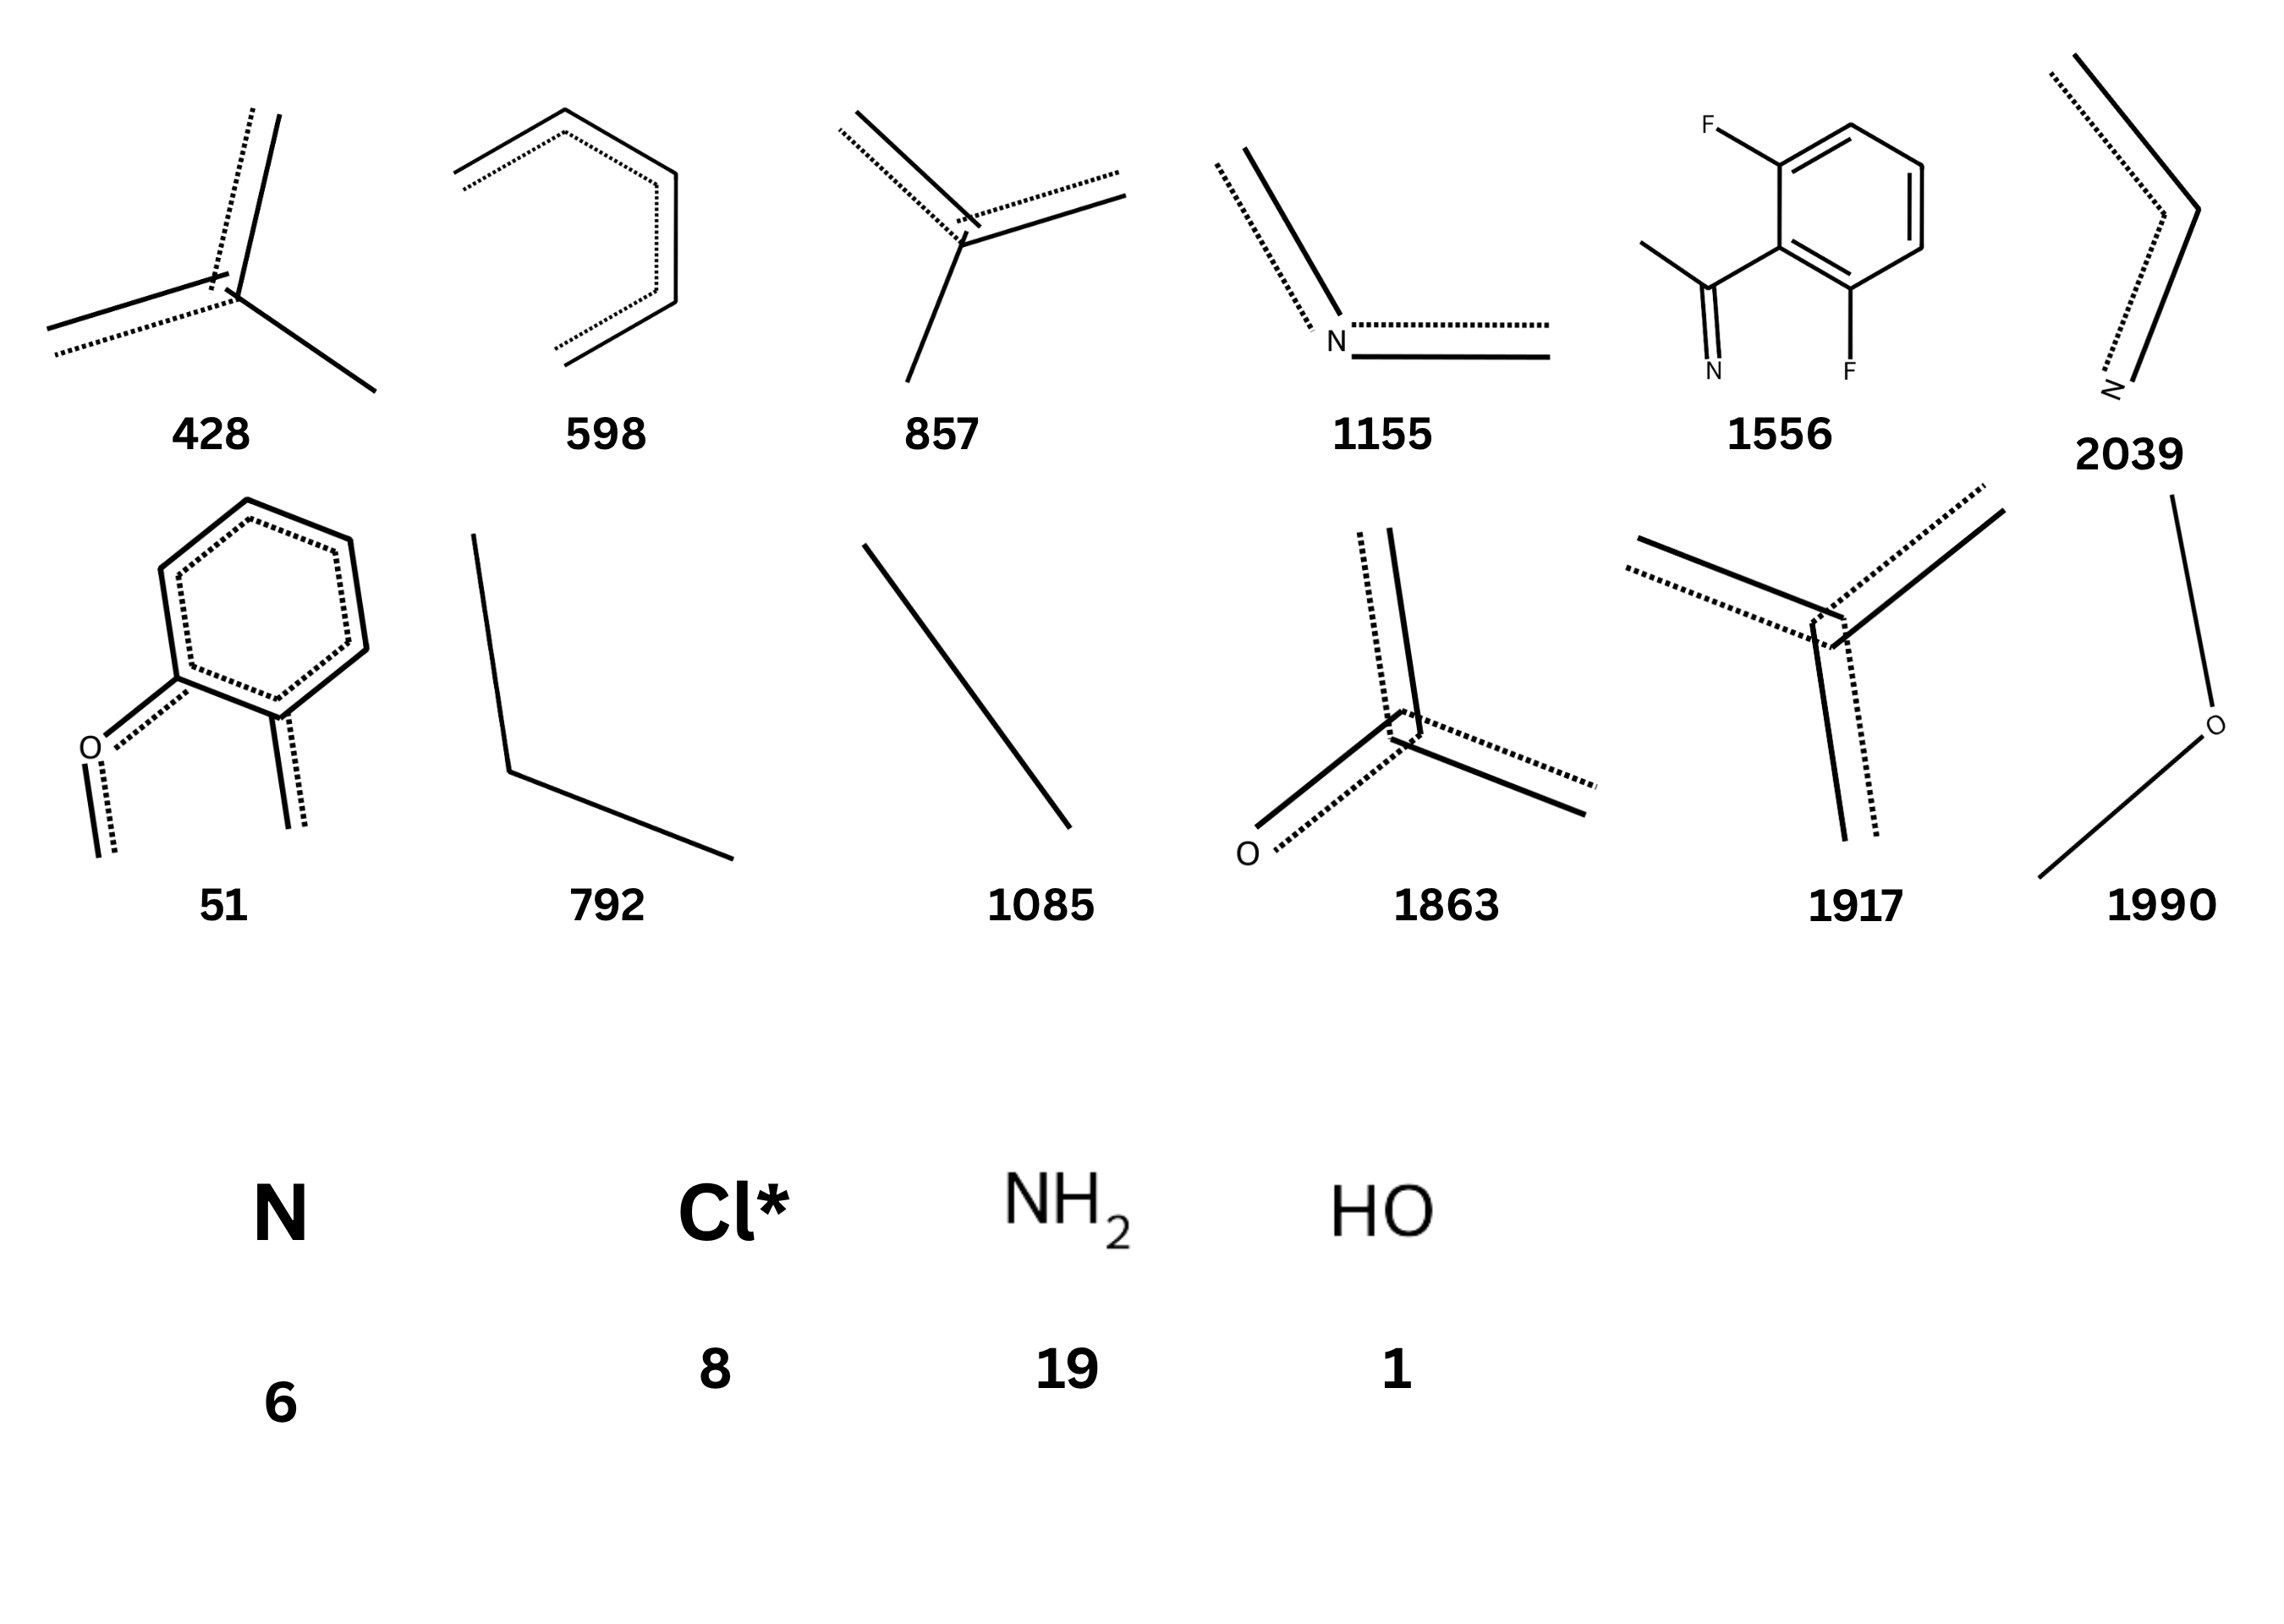
\includegraphics[width=0.8\textwidth]{mostcommonbitv2.png}
		\vspace{-0.3cm}
		
		\parbox{\textwidth}{\centering \footnotesize \textbf{*} Can be interpreted as other electronegative atoms/functional groups.}
		
		\vspace{0.3cm}
		\caption{Most common bits visualization:CSBC}
		\label{fig:mostcombits}
	\end{minipage}
\end{figure}
\FloatBarrier
\subsection*{CBC-ML and CSBC-ML Development}

\begin{table}[h]
	\centering
	\small
	\renewcommand{\arraystretch}{1.2}
\resizebox{\textwidth}{!}{%
	\begin{tabular}{p{3.5cm} p{1.5cm} c c c c c c c}
		\hline
		\textbf{QSAR-ML Model} & \textbf{Phase} & \textbf{Accuracy} & \textbf{Precision} & \textbf{Recall} & \textbf{F1 Score} & \textbf{Specificity} & \textbf{FNR} & \textbf{FPR} \\
		\hline
		CSBC-ML-Logit & Training & 0.7061 & 0.6985 & 0.7279 & 0.7129 & 0.6842 & 0.2721 & 0.3158 \\
		& Testing  & 0.7092 & 0.6976 & 0.7285 & 0.7127 & 0.6842 & 0.2721 & 0.3158 \\
		CBC-ML-Logit  & Training & 0.6328 & 0.6290 & 0.6519 & 0.6403 & 0.6136 & 0.3481 & 0.3864 \\
		& Testing  & 0.6214 & 0.6134 & 0.6366 & 0.6248 & 0.6136 & 0.3481 & 0.3864 \\
		CBC-ML-XGB    & Training & 0.7299 & 0.7344 & 0.7222 & 0.7283 & 0.7376 & 0.2778 & 0.2624 \\
		& Testing  & 0.7206 & 0.7143 & 0.7260 & 0.7201 & 0.7152 & 0.2740 & 0.2848 \\
		CSBC-ML-XGB   & Training & 0.9560 & 0.9347 & 0.9808 & 0.9572 & 0.9312 & 0.0192 & 0.0688 \\
		& Testing  & 0.9488 & 0.9240 & 0.9770 & 0.9498 & 0.9212 & 0.0230 & 0.0788 \\
		CSBC-ML-RF    & Training & 0.9562 & 0.9348 & 0.9812 & 0.9574 & 0.9312 & 0.0188 & 0.0688 \\
		& Testing  & 0.9484 & 0.9233 & 0.9770 & 0.9494 & 0.9204 & 0.0230 & 0.0796 \\
		CBC-ML-RF     & Training & 0.7300 & 0.7346 & 0.7222 & 0.7284 & 0.7378 & 0.2778 & 0.2622 \\
		& Testing  & 0.7206 & 0.7143 & 0.7260 & 0.7201 & 0.7152 & 0.2740 & 0.2848 \\
		CSBC-ML-SVM   & Training & 0.9476 & 0.9283 & 0.9704 & 0.9489 & 0.9247 & 0.0296 & 0.0753 \\
		& Testing  & 0.9435 & 0.9239 & 0.9655 & 0.9442 & 0.9220 & 0.0345 & 0.0780 \\
		CBC-ML-SVM    & Training & 0.7300 & 0.7346 & 0.7222 & 0.7284 & 0.7378 & 0.2778 & 0.2622 \\
		& Testing  & 0.7206 & 0.7143 & 0.7260 & 0.7201 & 0.7152 & 0.2740 & 0.2848 \\
		\hline
	\end{tabular}
}
	\caption{Combined training and testing performance metrics of CBC-ML and CSBC-ML Models}
	\label{tab:combined_metrics}
\end{table}

\begin{figure}[h] % 'h' places the figure approximately here
	\centering
	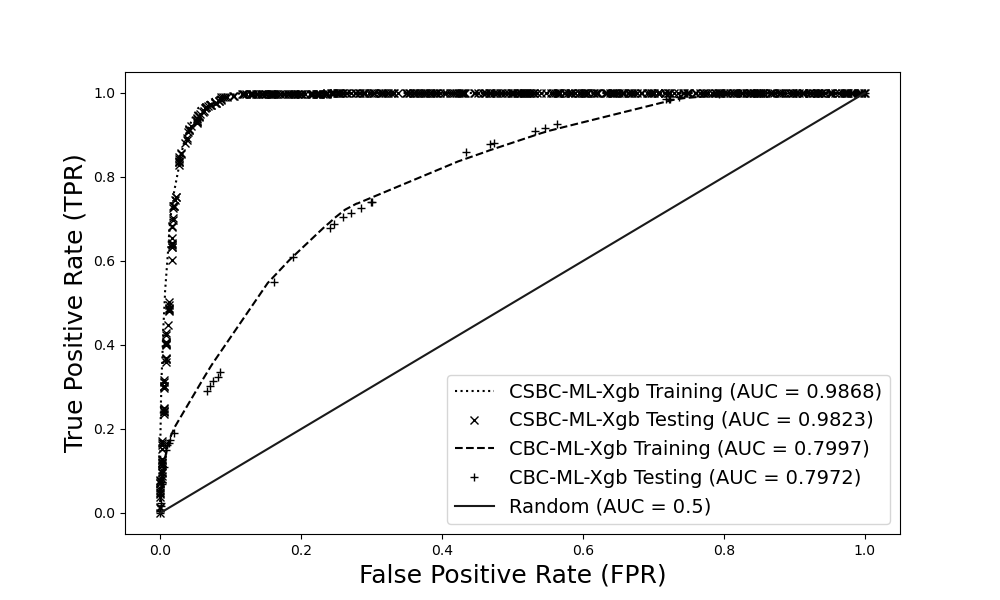
\includegraphics[width=0.8 \textwidth]{csbc_cbc_xgb.png} % Replace with your image filename
	\caption{Comparative summary of CSBC-ML-XGB and CBC-ML-XGB: ROC Curve}
	\label{fig:model_comparison_roc} % Optional: use \label for referencing
\end{figure}

\begin{figure}[h] % 'h' places the figure approximately here
	\centering
	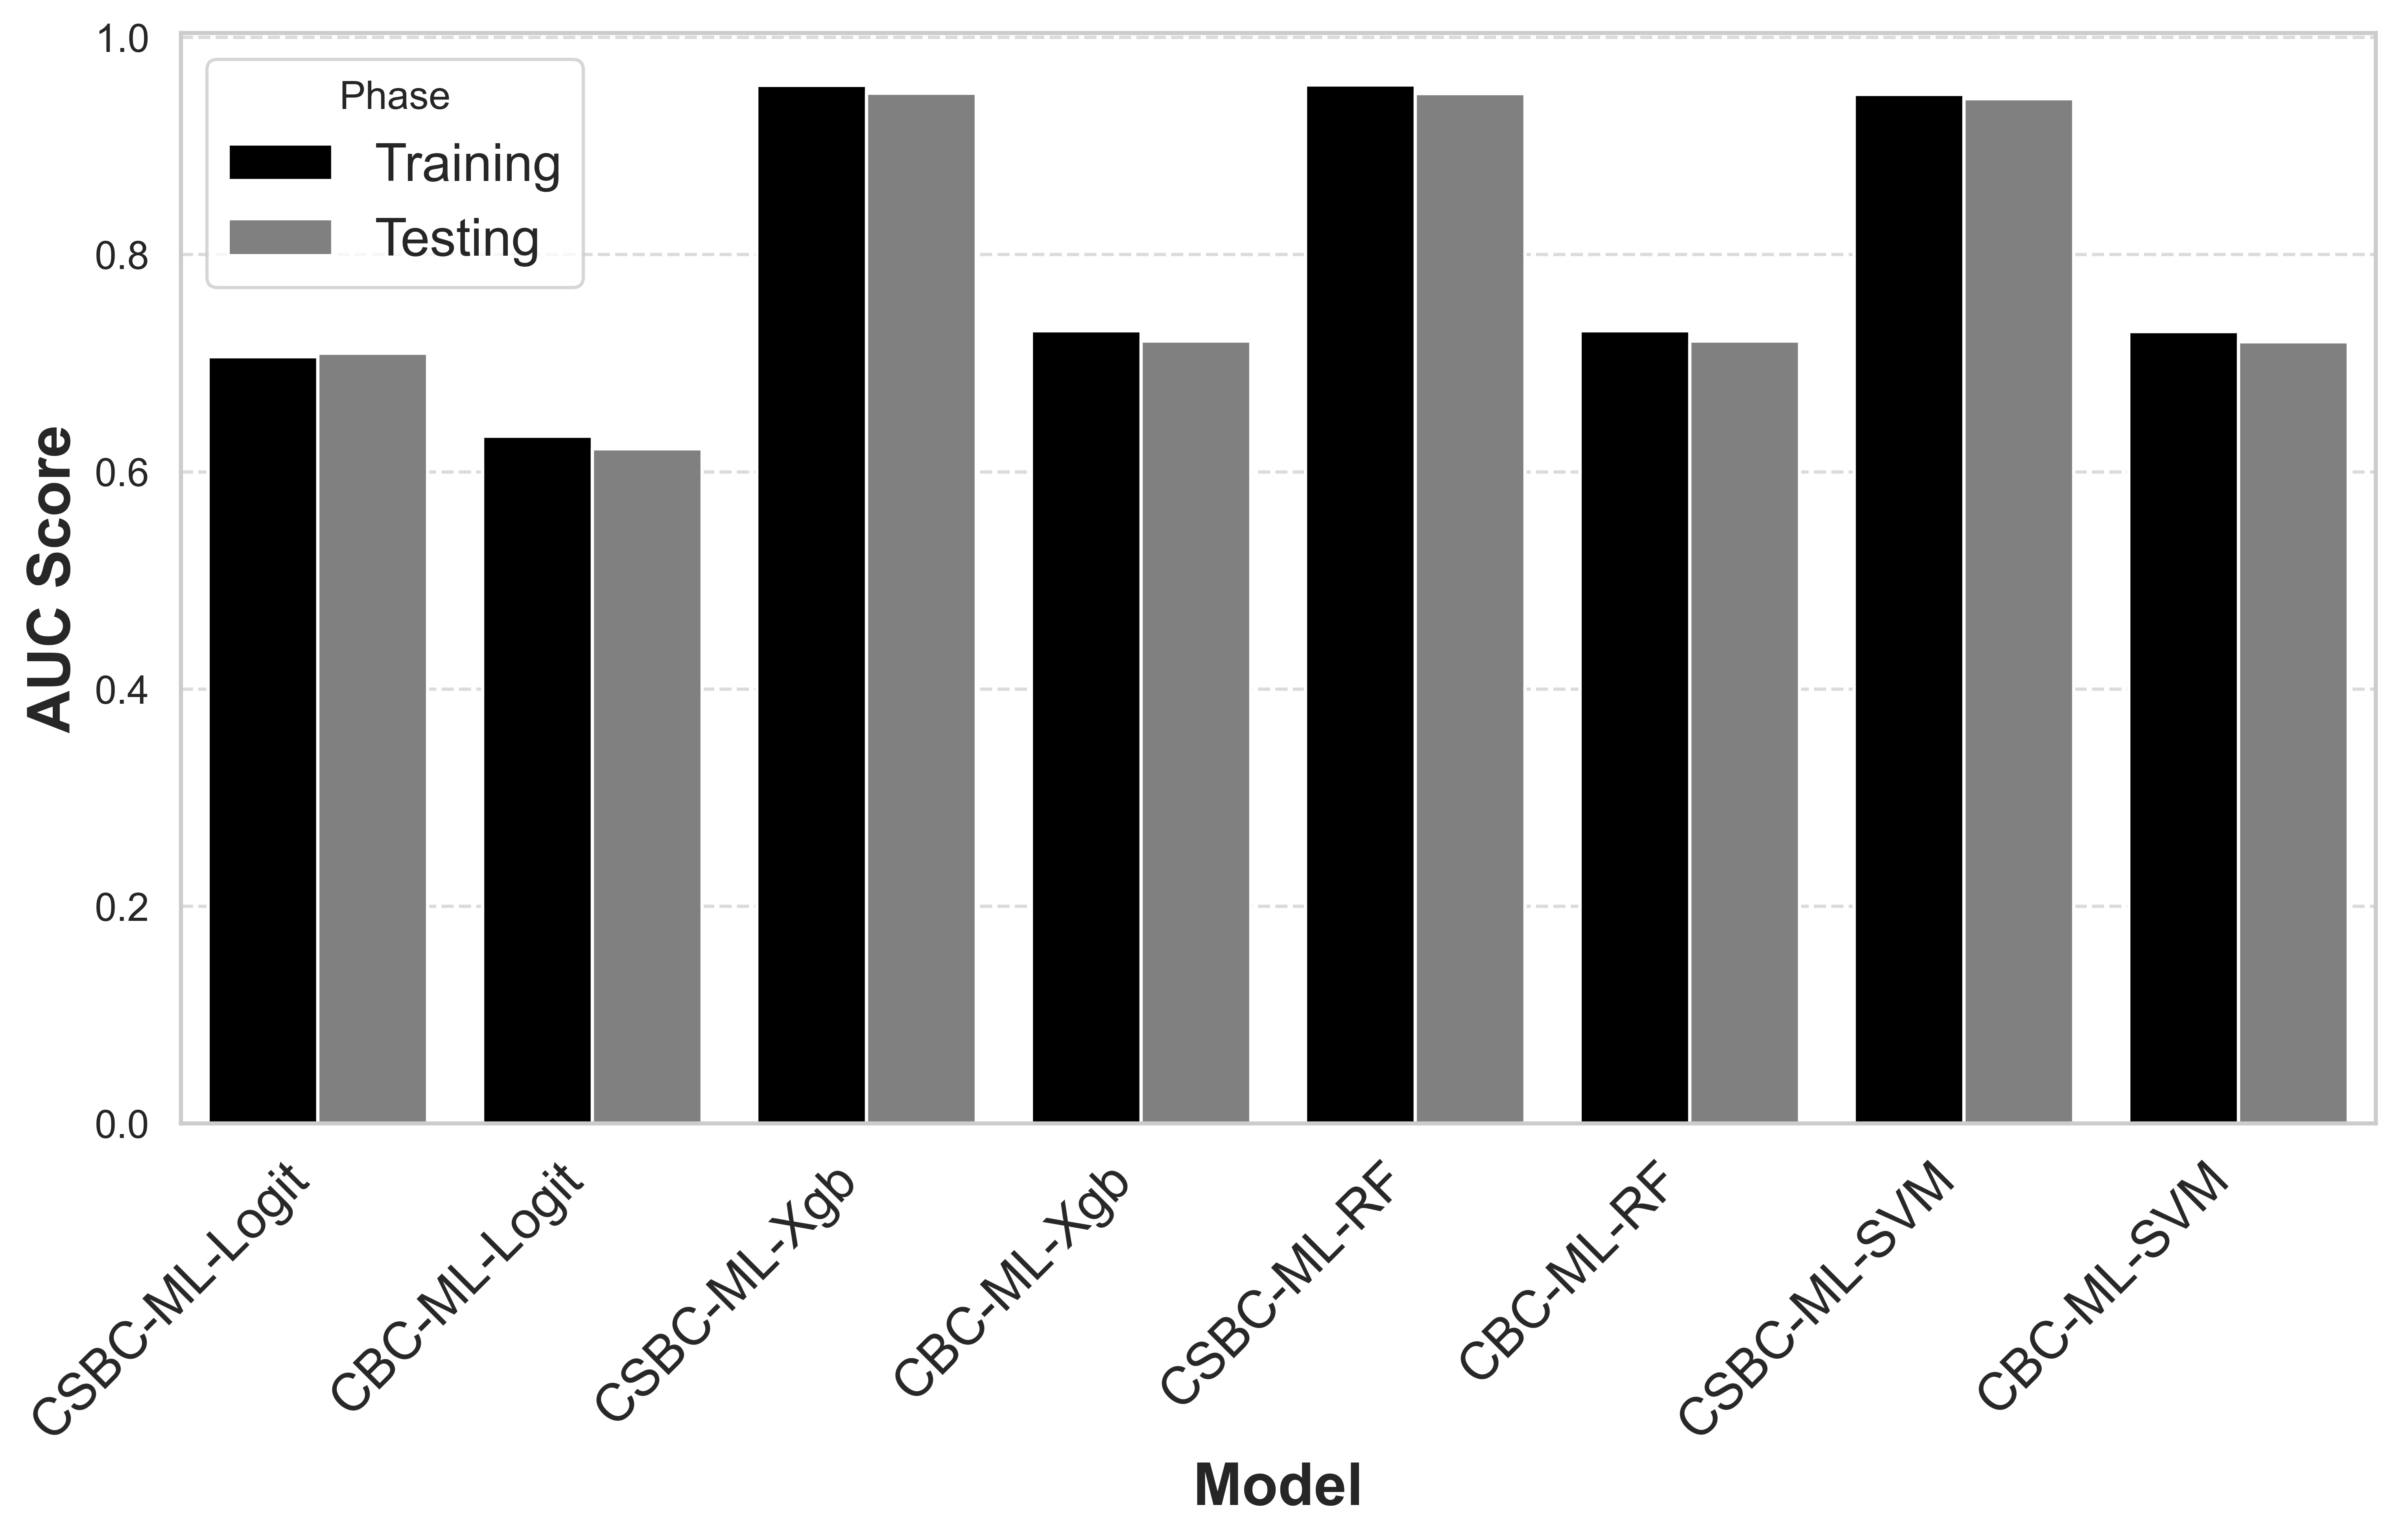
\includegraphics[scale=0.6]{auc_comparisonbw.png} % Replace with your image filename
	\caption{Comparative summary of CSBC-ML and CBC-ML: AUC Scores}
	\label{fig:model_comparison_auc} % Optional: use \label for referencing
\end{figure}

Logit models of CSBC produced an average of 70 \% in terms accuracy, recall, f1 and AUC score, together with FNR and FPR of 27 \% and 31 \% respectively. The same metrics for CBC logit models were found to be 63 \%, 34 \% and 38 \%, respectively (\autoref{tab:combined_metrics}). For XGB, RF AND SVM models, results revealed that CBC produced an average of 70\% for accuracy, recall, f1 and AUC score, 30 \% FNR and FPR while CSBC had an average of 94 \% in accuracy, 1 \% FNR and FPR, 98 \% recall, f1 and AUC score. CSBC models appeared to excellently classify activity against HCT-116, and it has a strong ability to generalize unknown data with minimal false predictions. On the other hand, CBC models have moderate predictive capacity and might suffer false predictions when unknown data increases. Overall, it was observed that CSBC models significantly outperforms CBC models in terms of confusion matrix parameters and AUC score. (\autoref{tab:combined_metrics}, \autoref{fig:model_comparison_auc}). The ROC curves showed that all the CBC-ML models suffered from over-fitting, whereas CSBC-ML models showed good fit even with unknown data. This suggests that CSBC-ML might be robust against increasing data set. \autoref{fig:model_comparison_roc} shows a sample comaparison of CSBC-ML and CBC-ML models. 


